%!TEX root = ../thesis.tex
% Spellchecker ignore
% cSpell:ignore Lett, detuned, nano, retroreflection, includegraphics, ifpdf, graphicspath, Rauschenbeutel, nanowaveguides, microresonator, signicant, nanofiber, textasciitilde, autoref
%*******************************************************************************
%****************************** Introduction ***********************************
%*******************************************************************************

\chapter*{Introduction}

% **************************** Define Graphics Path **************************
\ifpdf{}
    \graphicspath{{Introduction/Figs/Raster/}{Introduction/Figs/PDF/}{Introduction/Figs/}}
\else
    \graphicspath{{Introduction/Figs/Vector/}{Introduction/Figs/}}
\fi

\begin{figure}[hb]
    \centering
    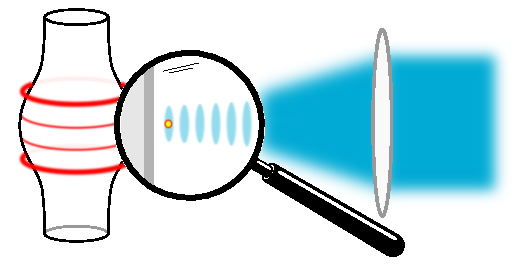
\includegraphics[width=0.6\textwidth]{resonator_trap}
    \caption{\label{fig:resonator_trap} Schematic representation of a WGM 
    resonator and a optical dipole trap}
\end{figure}
One of Prof.\ Rauschenbeutel projects uses a novel type of whispering-gallery-mode (WGM)
resonator interfaced via nanowaveguides and coupled to single Rubidium atoms to 
carry out experiments in the realm of Cavity Quantum Electrodynamics. The WGM 
resonator is a so-called bottle-microresonator (BMR) manufactured from a standard 
optical glass fiber in a heat and pull process. The light is radially confined 
inside the resonator by total internal reflection and propagates along the 
circumference of the resonator. In such a structure, a signicant fraction of the 
light field propagates in the evanescent field. By overlapping this field with 
the evanescent field of an optical nanofiber, light can be coupled into and out 
of the resonator very efficiently. Due to the extremely low absorption of silica 
(and low surface roughness) we can produce bottle-resonators with ultra-high 
optical Q-factor exceeding 10\(^{8}\). Rubidium atoms are delivered to the 
resonator using an atomic fountain. When the atoms enter the vicinity of the WGM, 
and they are in the evanescent field they can be strongly coupled to the light. 
For the moment the \(^{85}Rb\) atoms are only flying by the resonator for 
\textasciitilde{}\SI{2}{\micro\second}. Moreover the distance between the 
resonator and the atom is not controlled. This uncertainty induces fluctuations
on the atom-resonator coupling from shot to shot and limits the efficiency of the
different devices demonstrated with the setup. The short duration of the atom
light interaction also prevents the manipulation of the atomic state, necessary
for the realization of complex quantum information protocols such as two photon
gates~\cite{PhysRevLett.92.127902}. The solution would be to trap the atom at the
vicinity of the BMR\@. The choice made to trap the atom is to use a dipole trap 
created from the retroreflection of a focused beam on the resonator surface 
inspired from~\cite{Thompson1202} (see Fig.~\ref{fig:resonator_trap}). Due to the 
experiment configuration, the trap can not be loaded from a dense cloud, but only 
from the atoms flying next to the resonator, which have a non-zero velocity, which 
further implies that a big trap depth is needed. The usual dipole traps are built 
with lasers detuned from the transition between the ground and the first excited 
state. But this would create a trap too far from the resonator and thus in this 
thesis, we discuss the possibility to realise a trap detuned from the second exited 
state of \(^{85}\)Rb which has transitions at \(\lambda \approx \SI{420}{\nano\meter} \).
In this thesis, we will also evaluate the parameters needed for such a trap, and 
then report on an absorption spectroscopy measurement leading to the estimation 
of the saturation intensity of the \(5S_{1/2}\) to \(6P_{3/2}\) transition.